\section{Spektren aus der Literatur}
\label{sec:ref-spektren}
	
	\urldef{\refNa}\url{https://lexieslogofphysics.files.wordpress.com/2013/02/na22.jpg}
	\urldef{\refCs}\url{https://lexieslogofphysics.files.wordpress.com/2013/02/cs137.jpg}
	\urldef{\refEu}\url{http://www-np.ucy.ac.cy/radio_isotopes/wwwen/gamma/Eu152.png}

	\begin{figure}[hp]
		\centering
		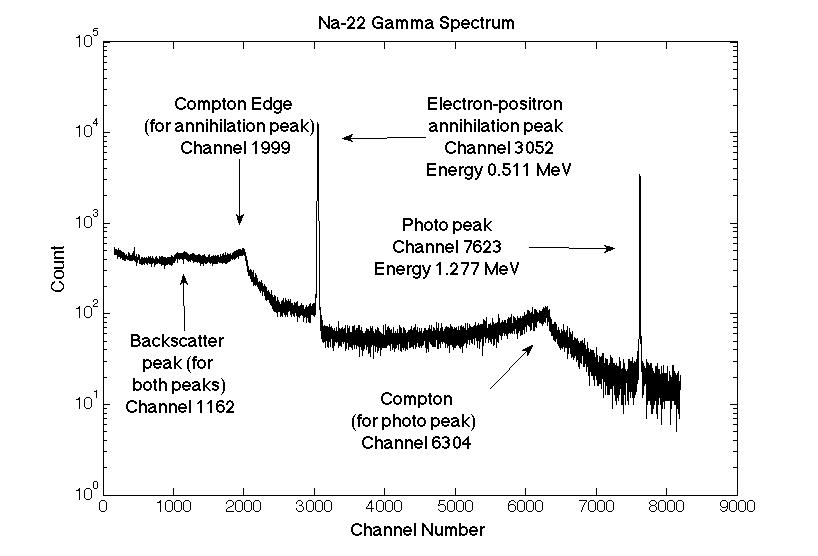
\includegraphics[scale=0.3]{ref/na22.jpg}
		\caption{$\gamma$-Spektrum einer $\prescript{22}{}{\m{Na}}$-Quelle \\ Quelle: \refNa}
		\label{fig:ref-na-22}
	\end{figure}
	\begin{figure}[hp]
		\centering
		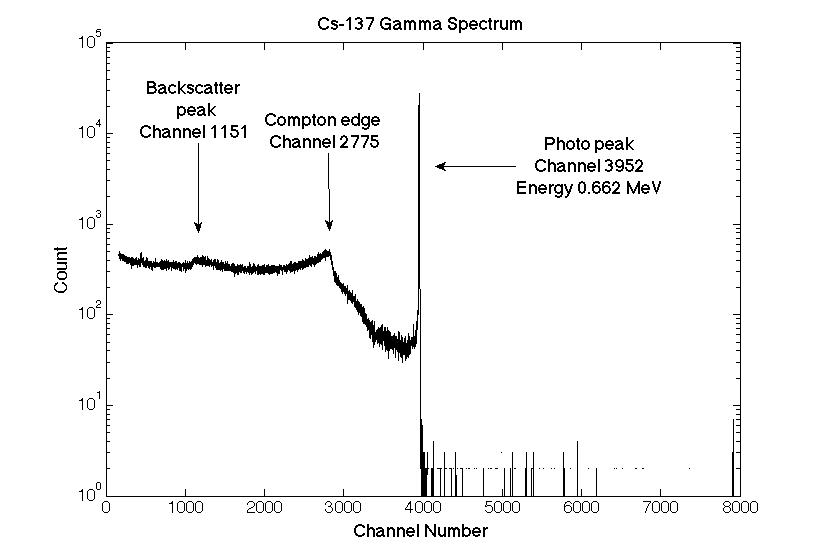
\includegraphics[scale=0.3]{ref/cs137.jpg}
		\caption{$\gamma$-Spektrum einer $\prescript{137}{}{\m{Cs}}$-Quelle \\ Quelle: \refCs}
		\label{fig:ref-cs-137}
	\end{figure}
	\begin{figure}[htb]
		\centering
		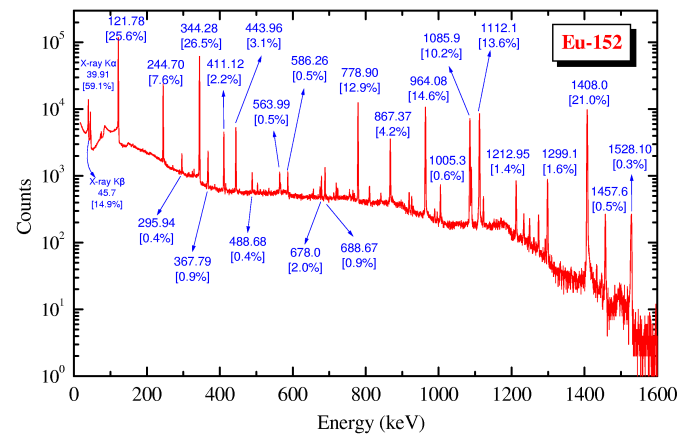
\includegraphics[scale=0.5]{ref/Eu152.png}
		\caption{$\gamma$-Spektrum einer $\prescript{152}{}{\m{Eu}}$-Quelle \\ Quelle: \refEu}
		\label{fig:ref-eu-152}
	\end{figure}

% section ref-spektren